\section{August 28, 2026}

We continue the study of one-step methods, focusing on consistency,
examples, and convergence. Let
\[
  t_0<t_1<\cdots<t_N,
  \qquad
  \tau_n=t_{n+1}-t_n,
\]
where $t_n$ is a time level and $\tau_n$ is the corresponding step size.
We use $x(t_n)$ for the exact solution and $x_n$ for its numerical
approximation:
\[
  x(t_n)\approx x_n.
\]

\begin{center}
  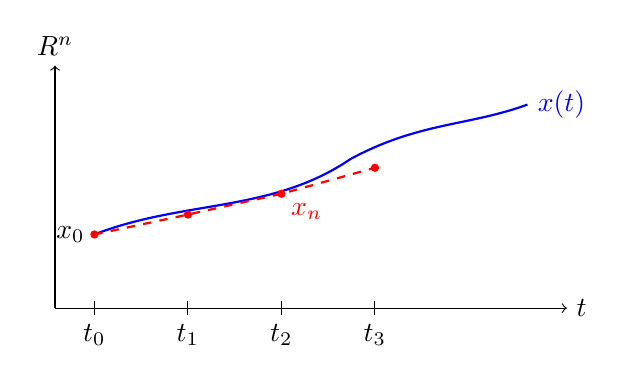
\begin{tikzpicture}[x=1.25cm,y=1.1cm]
    \draw[->] (0,0) -- (5.2,0) node[right] {$t$};
    \draw[->] (0,0) -- (0,2.8) node[above] {$\bb{R}^n$};
    \draw[blue,thick]
      (0.4,0.85) .. controls (1.3,1.25) and (2.2,1.10) ..
      (3.0,1.72) .. controls (3.7,2.15) and (4.2,2.10) ..
      (4.8,2.35) node[right] {$x(t)$};
    \draw[red,thick,dashed]
      (0.4,0.85) -- (1.35,1.08) -- (2.3,1.32) -- (3.25,1.62);
    \foreach \a/\b/\lab in {0.4/0.85/0,1.35/1.08/1,
                              2.3/1.32/2,3.25/1.62/3} {
      \draw (\a,0.08) -- (\a,-0.08) node[below] {$t_{\lab}$};
      \fill[red] (\a,\b) circle (1.5pt);
    }
    \node[left] at (0.4,0.85) {$x_0$};
    \node[red,below right] at (2.3,1.32) {$x_n$};
  \end{tikzpicture}
\end{center}

A one-step method advances the numerical solution by a map
\begin{equation}\label{eq:one-step-map-aug-28}
  x_{n+1}=\Psi^{t_{n+1},t_n}(x_n).
\end{equation}
Thus the exact and numerical solutions at $t_n$ can be written as
\begin{align*}
  x(t_n)
  &=\Phi^{t_n,t_{n-1}}\circ\cdots\circ
    \Phi^{t_2,t_1}\circ\Phi^{t_1,t_0}(x_0),\\
  x_n
  &=\Psi^{t_n,t_{n-1}}\circ\cdots\circ
    \Psi^{t_2,t_1}\circ\Psi^{t_1,t_0}(x_0).
\end{align*}

\subsection{Methods obtained from quadrature}

The integral form of the ODE over one step is
\begin{equation}\label{eq:one-step-integral-aug-28}
  x(t_{n+1})
  =x(t_n)+\int_{t_n}^{t_{n+1}}f(s,x(s))\,ds.
\end{equation}
Different quadrature approximations of this integral produce different
one-step methods.

\subsubsection{Forward Euler method}

Using the left endpoint in \eqref{eq:one-step-integral-aug-28} gives
\[
  x(t_{n+1})
  \approx x(t_n)+\tau_n f(t_n,x(t_n)).
\]
Replacing the exact solution values by numerical approximations yields
\begin{equation}\label{eq:forward-euler-aug-28}
  x_{n+1}=x_n+\tau_n f(t_n,x_n)
  =\Psi_{\mathrm{FE}}^{t_{n+1},t_n}(x_n).
\end{equation}

\subsubsection{Backward Euler method}

Using the right endpoint instead gives
\[
  x(t_{n+1})
  \approx x(t_n)+\tau_n f(t_{n+1},x(t_{n+1})).
\]
The resulting method is
\begin{equation}\label{eq:backward-euler-aug-28}
  x_{n+1}=x_n+\tau_n f(t_{n+1},x_{n+1})
  =\Psi_{\mathrm{BE}}^{t_{n+1},t_n}(x_n).
\end{equation}
Because $x_{n+1}$ occurs on both sides, backward Euler requires the
solution of a fixed-point problem at each step.

\subsubsection{A predictor--corrector method}

The trapezoidal rule suggests
\[
  x(t_{n+1})\approx x(t_n)
  +\frac{\tau_n}{2}
   \bigl(f(t_n,x(t_n))+f(t_{n+1},x(t_{n+1}))\bigr).
\]
We can first predict the right endpoint with forward Euler and then use
that prediction in the trapezoidal formula:
\begin{align}
  x_{n+1}^*
  &=x_n+\tau_n f(t_n,x_n),
    \label{eq:heun-predictor-aug-28}\\
  x_{n+1}
  &=x_n+\frac{\tau_n}{2}
    \bigl(f(t_n,x_n)+f(t_{n+1},x_{n+1}^*)\bigr).
    \label{eq:heun-corrector-aug-28}
\end{align}
This explicit two-stage scheme is also called Heun's method. Together,
the two stages define a one-step map
\[
  x_{n+1}=\Psi_{\mathrm{H}}^{t_{n+1},t_n}(x_n).
\]

\subsection{Local consistency error}

For a numerical one-step map $\Psi$, define its \emph{local error}, or
\emph{consistency error}, at $(t_n,x)$ by
\begin{equation}\label{eq:local-error-aug-28}
  \mathcal{E}_n(x)
  =\Phi^{t_{n+1},t_n}(x)-\Psi^{t_{n+1},t_n}(x).
\end{equation}
Here the exact and numerical steps start from the same value $x$ at
time $t_n$.

\begin{example}[Forward Euler]
  The Taylor expansion from \eqref{eq:flow-taylor-expansion} gives
  \begin{align*}
    \mathcal{E}_n^{\mathrm{FE}}(x)
    &=\Phi^{t_n+\tau_n,t_n}(x)
      -\bigl(x+\tau_n f(t_n,x)\bigr)\\
    &=\frac{\tau_n^2}{2}
      \bigl(f_t+f_xf\bigr)(t_n,x)+O(\tau_n^3)\\
    &=O(\tau_n^2).
  \end{align*}
\end{example}

\begin{example}[Backward Euler]
  Let
  \[
    y(\tau)=\Psi_{\mathrm{BE}}^{t_n+\tau,t_n}(x).
  \]
  The defining fixed-point equation is
  \[
    y(\tau)=x+\tau f(t_n+\tau,y(\tau)).
  \]
  Differentiating this equation and evaluating at $\tau=0$ gives
  \[
    y'(0)=f(t_n,x),
    \qquad
    y''(0)=2\bigl(f_t+f_xf\bigr)(t_n,x).
  \]
  Therefore,
  \[
    \Psi_{\mathrm{BE}}^{t_n+\tau_n,t_n}(x)
    =x+\tau_n f(t_n,x)
     +\tau_n^2\bigl(f_t+f_xf\bigr)(t_n,x)
     +O(\tau_n^3).
  \]
  Comparing this with the exact flow expansion yields
  \begin{align*}
    \mathcal{E}_n^{\mathrm{BE}}(x)
    &=-\frac{\tau_n^2}{2}
      \bigl(f_t+f_xf\bigr)(t_n,x)+O(\tau_n^3)\\
    &=O(\tau_n^2).
  \end{align*}
\end{example}

\subsection{Global error and convergence}

The \emph{global error} at $t_n$ is
\begin{equation}\label{eq:global-error-aug-28}
  e_n=x_n-x(t_n).
\end{equation}
The local errors accumulate as the method marches forward in time. On a
fixed time interval there are approximately $1/\tau$ steps of size
$\tau$, so one generally loses one power of $\tau$ when passing from
local to global error:
\[
  \mathcal{E}_n=O(\tau^{p+1})
  \quad\Longrightarrow\quad
  e_n=O(\tau^p).
\]
More generally, with
\[
  h=\max_{0\leq n<N}\tau_n,
\]
a stable one-step method with local error $O(h^{p+1})$ has global error
$O(h^p)$ under the usual smoothness assumptions. Thus both forward and
backward Euler have local error of order two and global order one.
